\documentclass[../../main.tex]{subfiles}

\graphicspath{{\subfix{../../immagini/}}}

\begin{document}
    Nell'ambito dell'apprendimento supervisionato, come brevemente introdotto nello scorso paragrafo, l'obiettivo è, una volta identificata la classe del problema su cui voglio lavorare, progettare un agente in grado di risolvere tale problema, nello specifico l'agente incaricato avrà a disposizione un dataset, che prende il nome di insieme d'addestramento, o training set, ossia un insieme di elementi etichettati su cui fare apprendimento.

    Formalmente, dato un insieme $X$ contenente gli oggetti su cui effettuare le predizioni, e $Y$ contenente le relative etichette, un training set è composto da $N$ elementi nella forma:
    \[(\boldsymbol{x_1}, y_1), (\boldsymbol{x_2}, y_2), \dots, (\boldsymbol{x_N}, y_N),\]
    con ogni etichetta generata da una funzione ignota $y = f(\boldsymbol{x})$, l'obiettivo è trovare una funzione $h$, detta funzione d'ipotesi, o modello, che approssimi in modo accettabile la funzione $f$. È importante notare come ognuno degli elementi del dataset $\boldsymbol{x}$ sia un vettore di $n$ elementi, ognuno di questi elementi prende il nome di caratteristica, o feature.

    L'obiettivo è quindi ricercare nello spazio delle possibili funzioni d'ipotesi una che approssimi la funzione $f$ sui dati noti, e che sia anche estendibile a esempi non appartenenti al dataset. Quando questo accade si dice in questo caso che $h$ è in grado di generalizzare.

    Esistono diverse classi di funzione d'ipotesi, tra cui:
    \begin{itemize}
        \item funzioni lineari,
        \item funzioni polinomiali grado N,
        \item funzioni sinusoidali,
        \item funzioni esponenziali.
    \end{itemize}

    A prescindere dal tipo di classe utilizzata, la funzione avrà una serie di parametri, o pesi. Prendendo come esempio la classe di funzioni lineari, questa ha una forma del tipo:
    \[ h(\boldsymbol{x}) = w_0 + w_1x_1 + \dots + w_nx_n .\]
    La funzione $h$ andrà ad approssimare una specifica funzione $f$ trovando il giusto valore del vettore di parametri $\boldsymbol{w}$, l'obiettivo quindi è trovare l'insieme di parametri che meglio descrive i dati presenti nel training set, questa operazione prende il nome di fitting. 

    A seconda di come la funzione $f$ è definita esistono due principali tipi di apprendimento supervisionato: nel caso in cui $f$ abbia come codominio $\mathbb{R}$ si parla di un problema di \textit{regressione}, se invece $f$ ha un codominio con un numero discreto e finito di elementi (quindi assegna un'etichetta ad ogni elemento dell'insieme di training) allora si parla di problema di \textit{classificazione}.

    Esistono in generale diversi algoritmi per le due tipologie di problemi appena descritte che differiscono principalmente per la loro espressività, ovvero la capacità di rappresentare determinati pattern di dati. Importante notare come molti algoritmi possano essere sfruttati sia nell'ambito della classificazione che in quello della regressione.

    Vengono ora introdotti brevemente, a scopo esemplificativo, la \textit{regressione lineare} per problemi di regressione, e la \textit{regressione logistica} per problemi di classificazione. Nel prossimo paragrafo vengono invece introdotte le \textit{reti neurali}, utilizzate poi negli esperimenti sui filtri.

    \subsubsection{Regressione}

    Nel caso della regressione la funzione $f$ da approssimare è una funzione con codominio continuo, come già accennato in precedenza sono diversi i metodi utilizzabili in problemi di questo tipo, come ad esempio \textit{regressione lineare, random forest, ..., support vector machines}. Questi vari approcci si differenziano principalmente per la complessità della funzione $h$ con conseguenti differenze nelle capacità di approssimazione di $f$.

    \begin{figure}[H]
        \centering
        \begin{subfigure}[t]{0.49\textwidth}
            \centering
            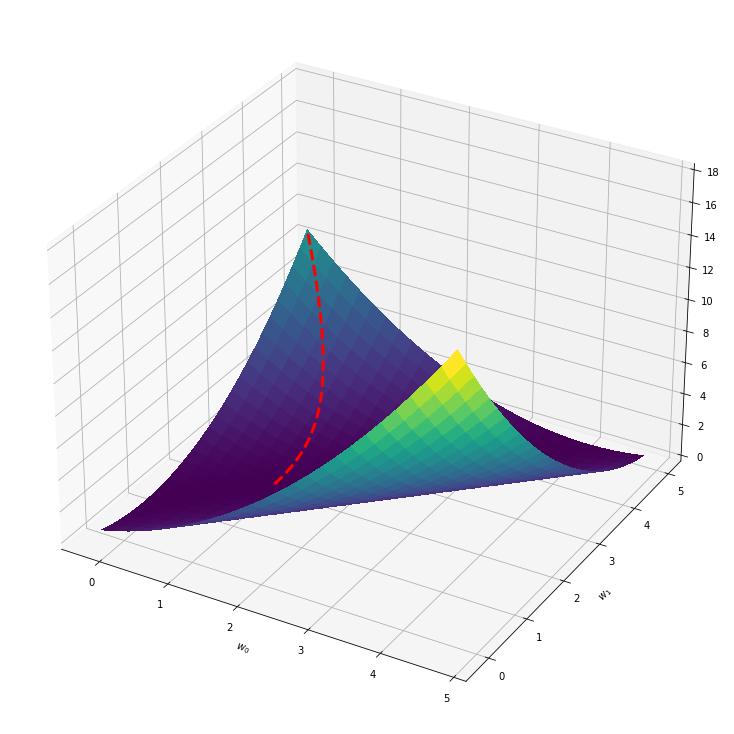
\includegraphics[width=\textwidth]{immagini/4_1/loss_function.png} 
            \caption{Grafico di un generica funzione di perdita.}
            \label{fig:funzioneLoss}      
        \end{subfigure}
        \begin{subfigure}[t]{0.49\textwidth}
            \centering
            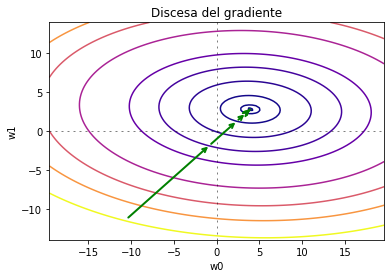
\includegraphics[width=\textwidth]{immagini/4_1/discesa_gradiente.png} 
            \caption{Curve di livello della funzione di perdita rappresentata nella figura a sinistra. Le frecce verdi mostrano la direzione e la lunghezza del passo compiuto per l'aggiornamento dei pesi ad ogni iterazione.}
            \label{fig:curveLivello}      
        \end{subfigure}
        \caption{Esempio del funzionamento dell'algoritmo del gradiente utilizzato per aggiornare il valore dei pesi: noto come il valore della funzione di perdita diminuisca all'aumentare del numero di iterazioni fino ad arrivare a convergenza}
        \label{fig:gradient_descent}
    \end{figure}

    Introduciamo ora uno dei metodi più semplici per ragionare su problemi di regressione: la regressione lineare.\\
    In questo caso la funzione d'ipotesi è definita come:
    \begin{equation}
        h(\boldsymbol{x}) = w_0 + w_1x_1 + w_2x_2 + \dots + w_nx_n = \boldsymbol{w^T x}.
        \label{eqn:linearhypotes}   
    \end{equation}

    Essendo $\boldsymbol{x}$  composto da $n$ elementi, la funzione $h$ contiene $n$ variabili, il problema prende in questo caso il nome di \textit{regressione lineare multi-variata}. L'idea è quella di sfruttare gli elementi dell'insieme di training a disposizione per trovare un vettore dei parametri $\boldsymbol{w}$ che permetta di minimizzare  una funzione, chiamata di perdita, che di fatto quantifica l'errore commesso dal modello.
    
    Posso definire la funzione di perdita in diversi modi, in questo caso considero una funzione di perdita quadratica:
    \begin{equation}
        L(\boldsymbol{w}) = \frac{1}{2N} \sum_{j=1}^N(y_j - h(\boldsymbol{x_j}))^2,
        \label{eqn:lossquadratica}
    \end{equation}
    dove il fattore $\frac{1}{2}$ viene aggiunto per eliminare il fattore $2$ nelle derivate presentate di seguito, rendendo più semplici i calcoli.

    Per minimizzare la funzione è necessario trovare dei parametri tali per cui la derivata di $L$, in funzione di tali parametri, sia pari a 0:
    \[\frac{\partial}{\partial w} L(\boldsymbol{w}) = 0.\]

    Nel caso della regressione lineare l'approccio più semplice è risolvere analiticamente la derivata al fine di ricavare un metodo generale con cui calcolare direttamente il valore di ognuno dei parametri. Prendendo ad esempio il caso della \textit{regressione univariata}, in cui $h$ è ad una sola variabile:
    \[h(x) = w_0 + w_1 x ,\]
    le derivate che si ottengono sono le seguenti, da cui posso poi ricavare i valori ottimi per i due pesi:
    \begin{equation}
        \begin{dcases}
            \frac{\partial}{\partial w_0} L(\boldsymbol{w}) = -\frac{1}{N}\sum_{j=1}^N\left(y_j - w_0 - w_1 x_j\right),\\
            \frac{\partial}{\partial w_1} L(\boldsymbol{w}) = -\frac{1}{N}\sum_{j=1}^N\left(y_j - w_0 - w_1 x_j\right) x_j.
        \end{dcases}   
        \label{eqn:regrLineareDer}      
    \end{equation}
    \[
    \rightarrow
    \begin{dcases}
        w_0 = & \frac{\sum_{j=1}^N y_j - w_1 \sum_{j=1}^N x_j}{N},\\
        w_1 = & \frac{N(\sum_{j=1}^N y_jx_j) - \sum_{j=1}^N y_j \sum_{j=1}^N x_j}{N(\sum_{j=1}^N y_j^2) - (\sum_{j=1}^N y_j)^2}. 
    \end{dcases}    
    \]
    Non sempre però un approccio di questo tipo è possibile: in molti casi infatti non esiste una soluzione in forma chiusa del sistema di equazioni , in casi di questo tipo solitamente si ricorre ad un approccio iterativo più generale con algoritmi che sfruttano il gradiente della funzione $L$, nel nostro caso utilizzeremo un algoritmo di \textit{discesa del gradiente} (Figura \ref{fig:gradient_descent}), in quanto l'obiettivo è di minimizzare il valore della perdita.

    Intuitivamente l'algoritmo lavora non più sulla perdita calcolata su tutto il dataset ma analizzando gli elementi di tale insieme uno alla volta ed aggiornando il valore dei pesi di conseguenza.\\
    Più formalmente, l'algoritmo \ref{alg:gradient_desc} mostra lo pseudocodice della procedura appena descritta, dove $\alpha$, chiamato learning rate, rappresenta la `forza' della modifica dei pesi ad ogni passo.

    \begin{algorithm}[H]
        \caption{Discesa del gradiente}\label{alg:gradient_desc}
        \begin{algorithmic}
            \State $\boldsymbol{w} \gets \text{inizializzazione}$
            \While{$\text{not convergenza}$}
            \State{$\boldsymbol{w} \gets \boldsymbol{w} - \alpha \nabla L(\boldsymbol{w})$}
            \EndWhile
        \end{algorithmic}
    \end{algorithm}  

    L'aggiornamento prevede quindi di calcolare prima il gradiente della perdita che viene poi utilizzato per modificare il valore dei parametri. Nella regressione univariata, sfruttando le derivate del sistema \ref{eqn:regrLineareDer}:
    \[
        \begin{dcases}
            w_0 \leftarrow w_0 - \alpha \frac{\partial}{\partial w_0} L(\boldsymbol{w})\\
            w_1 \leftarrow w_1- \alpha \frac{\partial}{\partial w_1} L(\boldsymbol{w})
        \end{dcases}
        \rightarrow
        \begin{dcases}
            w_0 \leftarrow w_0 + \alpha \frac{1}{N} \sum_{j=1}^N (y_j - h(x_j))\\
            w_1 \leftarrow w_1 + \alpha \frac{1}{N} \sum_{j=1}^N (y_j - h(x_j))x_j
        \end{dcases}
    \]
    Lo stesso ragionamento può essere fatto per la regressione multivariata, ottenendo la seguente regola di aggiornamento dei pesi:
    \[w_i \leftarrow w_i + \alpha \sum_{j=1}^N(y_j - h(\boldsymbol{x_j}))x_{j,i},\]
    dove $x_{j,i}$ indica l'$i$-esimo elemento del vettore $\boldsymbol{x_j}$.

    \subsubsection{Classificazione} 
    

    Se la funzione $f$ da approssimare ha un codominio discreto si parla di classificazione. Inoltre, a seconda del numero di elementi nel codominio di $f$ facciamo riferimento a diversi tipi di classificazione: se il dataset contiene esempi solamente di due etichette differenti si parla di classificazione \textit{binaria}, in caso contrario si parla di classificazione \textit{multiclasse}. Anche in questo caso sono diversi i metodi che vengono utilizzati, citandone alcuni: \textit{Regressione logistica, Naive-Bayes, ..., Alberi di Decisione}.
    
    Introduciamo ora uno dei metodi più semplici: la regressione logistica, ma mostriamo prima come sia possibile adattare la regressione lineare, introdotta nel paragrafo precedente, anche per problemi di classificazione sfruttando il concetto di soglia.

    \begin{figure}[H]
        \begin{subfigure}[]{0.49\textwidth}
            \centering
            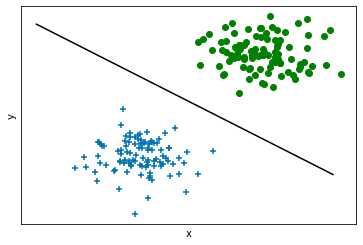
\includegraphics[width=\textwidth]{immagini/4_1/class_linearly_separable.png} 
            \caption{Esempio di dataset linearmente separabile}
            \label{fig:linearly_sep_classification}      
        \end{subfigure}
        \begin{subfigure}[]{0.49\textwidth}
            \centering
            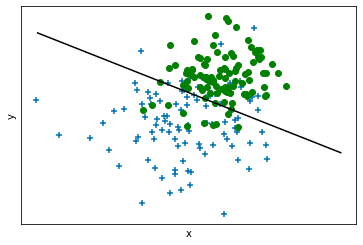
\includegraphics[width=\textwidth]{immagini/4_1/class_non_linearly_separable.png}    
            \caption{Esempio di dataset non linearmente separabile}
            \label{fig:non_linearly_sep_classification}    
        \end{subfigure}
        \caption{}
    \end{figure}

    Un modello lineare può essere utilizzato anche nel contesto dei problemi di classificazione: in Figura \ref{fig:linearly_sep_classification}, ad esempio,  è rappresentato un insieme di punti appartenenti a due etichette differenti, fornito un dataset di questo tipo l'obiettivo in un problema di classificazione è apprendere una funzione d'ipotesi $h$ che, dato un nuovo punto $x$, fornisca in output una predizione per l'etichetta $y$, l'obiettivo è ovviamente quello di avere globalmente delle buone predizioni. 
    
    In generale si definisce decision boundary il piano che separa i punti appartenenti a etichette differenti, se tale boundary è, come nell'esempio della figura, una linea retta si parla di classi linearmente separabili. 
    
    Per adattare l'approccio già citato per il caso della regressione al contesto della classificazione semplicemente introduco il concetto di soglia: riprendendo la funzione d'ipotesi definita nell'equazione \ref{eqn:linearhypotes}, che chiamiamo qui $z$:
    \[z(\boldsymbol{x}) = x_0 + w_1x_1 + \dots + w_nx_n,\]
    se dato un punto $\boldsymbol{x}$ questo assume un valore $> 0$ nella funzione $z$ allora $h(\boldsymbol{x}) = 1$ altrimenti $h(\boldsymbol{x}) = 0$. Formalmente, possiamo quindi pensare di passare il risultato di $z$ in una funzione soglia (Figura \ref{fig:threshold}) ed utilizzare il risultato di questa funzione come predizione dell'etichetta:
    \[h(\boldsymbol{x}) = \text{Soglia}(z(\boldsymbol{x})) \ \text{con} 
    \begin{dcases}
        \text{Soglia(y)} = 1 & \text{se} \ y \geq 0 \\
        \text{Soglia(y)} = 0 & \text{altrimenti} \\
    \end{dcases}\]
    Noto come definendo in questo modo il modello non sia però possibile aggiornare i pesi utilizzando lo stesso approccio adottato nel caso della regressione: il gradiente di $h$ è infatti sempre pari a 0 tranne nei punti in cui $\boldsymbol{w} \cdot \boldsymbol{x} = 0$, in cui però è indefinito.
    
    La soluzione è quella di utilizzare la percepron learning rule:
    \[w_i \leftarrow w_i + \alpha (y - h(\boldsymbol{x})) x_i, \]
    lavorando su problemi di classificazione binaria 0/1 questa regola intuitivamente aggiornerà i pesi solamente nel caso in cui il risultato del modello sia errato, infatti:
    \begin{itemize}
        \item se la predizione è corretta, i pesi non vengono aggiornati: $w_i \leftarrow w_i + \alpha \cdot 0 = w_i$.
        \item Se $y = 1$ ma $h(\boldsymbol{x}) = 0$ allora $w_i$ viene aumentato quando il relativo $x_i$ è positivo e diminuito quando è negativo, in questo modo il prodotto $\boldsymbol{w} \cdot \boldsymbol{x}$ aumenta e la funzione d'ipotesi viene di conseguenza corretta  verso il valore 1.
        \item Se $y = 0$ ma $h(\boldsymbol{x}) = 1$ allora $w_i$ viene diminuito quando il relativo $x_i$ è positivo e aumentato quando è negativo, in questo modo il prodotto $\boldsymbol{w} \cdot \boldsymbol{x}$ diminuisce e la funzione d'ipotesi viene di conseguenza corretta verso il valore 0.
    \end{itemize}
    Solitamente questa regola di apprendimento viene applicata un esempio alla volta, estraendo casualmente elementi dal dataset.

    \begin{figure}[H]
        \begin{subfigure}{0.5\textwidth}
            \centering
            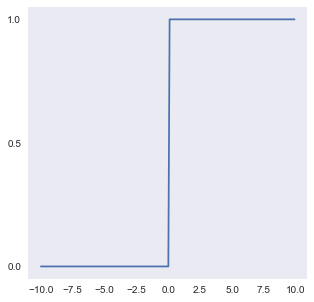
\includegraphics[width=\textwidth]{immagini/4_1/threshold.png} 
            \caption{Funzione Soglia}
            \label{fig:threshold}
        \end{subfigure}
        \begin{subfigure}{0.5\textwidth}
            \centering
            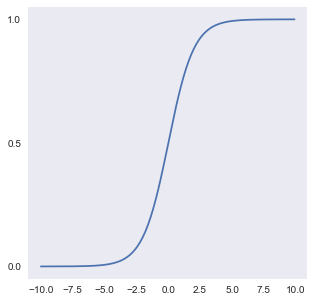
\includegraphics[width=\textwidth]{immagini/4_1/logistic.png}
            \caption{Funzione Logistica}
            \label{fig:logistic}
        \end{subfigure}
        \caption{Grafici della funzioni soglia e logistica.}
    \end{figure}

    Come appena mostrato quindi utilizzare l'output di un modello lineare come input di una funzione soglia permette di adattare l'approccio già utilizzato per il problema della regressione al contesto della classficazione, il principale lato negativo di utilizzare una funzione di questo tipo deriva dal fatto che non è differenziabile, un classificatore basato su una funzione di questo tipo inoltre fornisce sempre valori binari, anche quando il risultato è molto vicino al valore della soglia. Nella maggior parte delle situazioni una funzione di questo tipo non è ciò di cui abbiamo bisogno.

    Per i motivi appena descritti spesso si preferisce utilizzare una funzione logistica (Figura \ref{fig:logistic}), che intuitivamente corrisponde ad una versione rilassata della funzione soglia. Formalmente è definita come:
    \[ \text{Logistica}(y) = \frac{1}{1 + e^{-y}}, \]
    utilizzando come input il risultato del modello:
    \[h(\boldsymbol{x}) = \text{Logistica}(z(\boldsymbol{x})) = \text{Logistica}(\boldsymbol{w} \cdot \boldsymbol{x}) = \frac{1}{1 + e^{- \boldsymbol{w \cdot x}}} .\]
    Importante notare come l'output della funzione non sia più, come nella funzione soglia, un numero dell'insieme $\{0,1\}$, bensì un valore reale compreso nell'intervallo $[0, 1]$ che può essere interpretato come la probabilità che l'etichetta predetta per il punto $\boldsymbol{x}$ sia 1.

    La funzione logistica ha proprietà matematiche più vantaggiose rispetto alla funzione precedente, prima fra tutte la derivabilità su tutto il dominio, proprietà sfruttata per il processo di aggiornamento dei pesi, che prende il nome di \textit{regressione logistica}. 
    
    Non esiste, come nella regressione lineare, una soluzione in forma chiusa per trovare in modo analitico un valore per il vettore $\boldsymbol{w}$ che minimizzi la perdita, possiamo però ancora una volta sfruttare la discesa del gradiente. L'aggiornamento dei pesi avverrà quindi secondo la seguente formula:
    \[w_i \leftarrow w_i - \alpha \frac{\partial}{\partial w_i} L(\boldsymbol{w}).\]
    Considerando la funzione di perdita introdotta nell'equazione \ref{eqn:lossquadratica} ne calcolo la derivata, utilizzando come funzione d'ipotesi la funzione logistica, come definita poco sopra:
    \begin{align*}
        \frac{\partial}{\partial w_i} L(\boldsymbol{w}) &= -\frac{1}{N} \sum_{j=1}^N \left((y_j - h(\boldsymbol{x_j})) \cdot \frac{\partial}{\partial w_i} (y_j - h(\boldsymbol{x_j})) \right),\\
        &= -\frac{1}{N} \sum_{j=1}^N \left((y_j - h(\boldsymbol{x_j})) \cdot \frac{\partial}{\partial w_i} h(\boldsymbol{x_j}) \cdot x_{j,i} \right),\\
        &= -\frac{1}{N} \sum_{j=1}^N \left((y_j - h(\boldsymbol{x_j})) \cdot h(\boldsymbol{x_j}) \cdot (1 - h(\boldsymbol{x_j})) \cdot x_{j,i} \right).
    \end{align*}
    L'ultimo passaggio vale perchè la derivata parziale della funzione logistica è:
    \begin{align*}
        \frac{\partial}{\partial w_i} h(\boldsymbol{x_j}) &= \frac{\partial}{\partial w_i} \left(\frac{1}{1 + e^{-\boldsymbol{w}\cdot\boldsymbol{x}}}\right) = \frac{e^{-\boldsymbol{w}\cdot \boldsymbol{x}}}{\left(1 + e^{-\boldsymbol{w}\cdot \boldsymbol{x}}\right)^2}\\
        &= \frac{1}{1 + e^{-\boldsymbol{w}\cdot\boldsymbol{x}}} - \frac{1}{\left(1 + e^{-\boldsymbol{w}\cdot\boldsymbol{x}}\right)^2} = \frac{1}{1 + e^{-\boldsymbol{w}\cdot\boldsymbol{x}}}\left(1 - \frac{1}{1 + e^{-\boldsymbol{w}\cdot\boldsymbol{x}}}\right).
    \end{align*}

    Possiamo quindi riscrivere la formula per l'aggiornamento dei pesi:
    \begin{equation}
        w_i \leftarrow w_i + \alpha \sum_{j=1}^N \left((y_j - h(\boldsymbol{x_j})) \cdot h(\boldsymbol{x_j}) \cdot (1 - h(\boldsymbol{x_j})) \cdot x_{j,i} \right),
    \end{equation}
    dove il fattore $\frac{1}{N}$ è inglobato all'interno del learning rate $\alpha$.

    I metodi come la regressione lineare/logistica rimangono comunque fortemente limitati nel tipo di pattern dei dati che possono descrivere, per questo molto spesso si rendono necessari modelli più espressivi per  poter approssimare un determinato dataset, un esempio di questi modelli sono le \textit{reti neurali}, descritte nel paragrafo successivo.

\end{document}